\documentclass[14pt]{beamer}
\title[COJ:Java:01]{COJ :: Exception Handling}
\author[TS]{TalentSprint}
\institute[L\&D]{Licensed To Skill}
\date{Version 1.0.4}
\usefonttheme{serif}
\usecolortheme{orchid}
\usepackage{bookman}
\usepackage{hyperref}
\usepackage[T1]{fontenc}
\usepackage{graphicx}
\graphicspath{{../../Images/}}
\usepackage{listings}
\usepackage{framed, color}
\definecolor{shadecolor}{rgb}{0.7421875,0.7421875,0.7421875}
\beamertemplateballitem
\usebackgroundtemplate{
\includegraphics[width=\paperwidth]{TS-Logo.jpg}}
\lstset{language=Java,numbers=left, numberstyle=\tiny, numbersep=10pt, showstringspaces=false, breaklines=true,keepspaces=true, columns=flexible}
\begin{document}

\begin{frame}
  \titlepage
\end{frame}

\begin{frame}{Learning Objectives}
The content in this presentation is aimed to learn the following:
  \begin{itemize}
  \item Define Exception
  \item Differentiate Exception and Error
  \item Explain Types of exceptions
  \item Use try-catch-finally construct
  \item Use throws construct
 
 \end{itemize}
\end{frame}

\begin{frame}{Exception Handling}
 Define Exception:
 
Exception is a run-time error which arises during the execution of java program. The term exception stands for an ``exceptional event''.

What happens when an exception occur:
\begin{itemize}
 \item Exception are typically an event or conditions that arise during the execution which interrupt the normal flow of program
 \item Java Provides with exception handling mechanism using try and catch
 \item Exception handling is used to ensure graceful termination of program
\end{itemize}
\end{frame}

\begin{frame}{Exception Handling}
 Difference between Error and Exception:
 \textbf{Errors:}
 \begin{itemize}
  \item Error indicates serious problem that a reasonable application should not try to catch
  \item You cannot handle Error
  
 Example: JVM out of memory, Stack overflow
 \end{itemize}
\textbf{Exception:}
 \begin{itemize}
  \item Exception indicates conditions that a reasonable application might want to catch
  \item You can handle Exceptions
  
  Example: ArithmeticException
 \end{itemize}
\end{frame}

\begin{frame}{Exception Handling}
 Exception Hierarchy:
 \begin{figure}[H]
  \begin{center}
 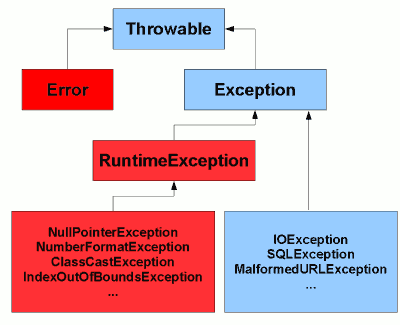
\includegraphics[scale=.8]{exception-heirarchy.png}  
  \end{center}

 \end{figure}
\end{frame}

\begin{frame}{Exception Handling}
 Types of Exceptions:
 
 There are two types of Exceptions:
\begin{enumerate}
 \item UnChecked Exceptions:
       These are the exceptions that are not checked at compile time
       All these exceptions are sub-classes for RuntimeException class
       
       Example: ArithmeticException, ArrayIndexOutOfBoundsException

\item Checked Exceptions:
      These are the exceptions that are checked at compile time
      These exceptions are sub-classes of Exception class and not RuntimeException class
      
      Example: IOException
\end{enumerate}
\end{frame}

\begin{frame}{Exception Handling}
 Exception Constructs:
 
 \begin{description}
  \item [try] This block encases any statements that might cause an exception to occur.
  \item [catch] This block(s)  provide a place to handle the exception thrown by the statements within a try block.
  \item [finally] The statements in the finally block are always executed. We can write resource clean up code here.
  \item [throw] Used to throw a specific exception from the program.
  \item [throws] Specifies which exceptions a given method can throw.
 \end{description}
\end{frame}

\begin{frame}{Exception Handling}
 Exception-Handling Blocks:
 \begin{figure}[H]
  \begin{center}
   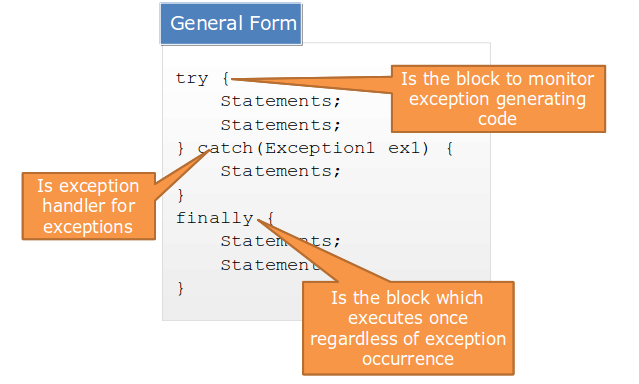
\includegraphics[scale=.4]{general-form.png}
  \end{center}

 \end{figure}
\end{frame}

\begin{frame}[fragile]{Exception Handling}
 Program without exception handler:
 \begin{lstlisting}[basicstyle=\tiny]
public class ExceptionDemo {
    public static void main(String[] args) {
        int i = 0, j = 10;
        int k = j / i;
        System.out.println("K is: " + k);
    }
}
\end{lstlisting}
\begin{block}{Output}
Exception in thread "main" java.lang.ArithmeticException: / by zero
at com.ts.exceptions.ExceptionDemo.main
\end{block}
\begin{block}{Note}
 The above code is without exception handling mechanism.
\end{block}
\end{frame}

\begin{frame}{Exception Handling}
 What happens when an exception occurs and program doesn't have exception handling code:
 \begin{itemize}
  \item When an exception occurs an object of the exception type is created first.
  \item This object contains the information about the exception like its type, message and when it occured.
  \item This object is handed over to runtime system which is called as throwing an exception.
  \item Now the runtime system searches for a block of code that can handle the exception.
  \item When an appropriate handler is not found, the runtime system prints default message and terminates.
 \end{itemize}
\end{frame}

\begin{frame}[fragile]{Exception Handling}
Program with exception handler:
\begin{lstlisting}
public class ExceptionDemo {
    public static void main(String[] args) {
        try {
            int i = 0, j = 10;
            int k = j / i;
            System.out.println("K is: " + k);
        } catch(ArithmeticException ae) {		
            System.out.println(``diving by zero'');
        }
    }
}
\end{lstlisting}
\end{frame}

\begin{frame}{Exception Handling}
 What happens when an exception occurs and program have exception handling code:
 \begin{itemize}
  \item When an exception occurs an object of the exception type is created first.
  \item This object contains the information about the exception like its type, message and when it occurred.
  \item This object is handed over to runtime system which is called as throwing an exception.
  \end{itemize}
  \end{frame}
  
\begin{frame}{Exception Handling}
  What happens when an exception occurs and program have exception handling code:
  \begin{itemize}
  \item Now the runtime system searches for a block of code that can handle the exception. This block of code is called exception        handler.
  \item An exception handler is considered appropriate if the type of the exception object thrown matches the type that can be          handled by the handler.
  \item If the match is found, then the appropriate exception handler block is executed.
 \end{itemize}
\end{frame}

\begin{frame}[fragile]{Exception Handling}
  Multiple catch blocks:
  \begin{shaded}
   \begin{lstlisting}[numbers=none, basicstyle=\tiny]
try {
    Statements;
    Statements;
} catch(Exception1 ex1) {
    Statements;
} catch(Exception1 ex1) {
    Statements;
}
 \end{lstlisting}
 \end{shaded}
 \begin{itemize}
  \item The statements within a single try block can generate different kind of exceptions
  \item So its  a good programming practice, to write a dedicated catch block for each kind of exception
 \end{itemize}
\end{frame}

\begin{frame}[fragile]{Exception Handling}
   The \lstinline!finally! block
   \begin{itemize}
    \item The statements in the finally block are always executed
    \item This is a good place to write clean up code like releasing file objects etc
   \item The statements within finally will execute if any exception occurs or not
  \begin{block}{Syntax}
   \begin{lstlisting}[numbers=none]
finally {
    Statements;
}  
   \end{lstlisting}

  \end{block}

 \end{itemize}
\end{frame}

\begin{frame}[fragile]{Exception Handling}
Program generating checked Exception:
\begin{block}{Example}
 \begin{lstlisting}
public class ExceptionDemo {
    public static void main(String[] args) {
        Thread.sleep(100);
    }
}
\end{lstlisting}

\end{block}
\end{frame}
\begin{frame}[fragile]{Exception Handling}
Program generating checked Exception:
After compilation:
\begin{verbatim}
javac ExceptionDemo.java 
ExceptionDemo.java:3: error: unreported 
  exception InterruptedException; 
  must be caught or declared to be 
  thrown Thread.sleep(100);
                     ^
1 error
  
\end{verbatim}
\end{frame}

\begin{frame}[fragile]{Exception Handling}
 \lstinline!throws! keyword:
 \begin{itemize}
  \item used to delegate the responsibility of exception handling to the caller method
  \item used to throw checked exceptions out of a method
 \end{itemize}
 \begin{block}{Usage of throws}
  \begin{lstlisting}
public class ExceptionDemo {
    public static void main(String[] args) throws Interrupted Exception {
        Thread.sleep(100);		
    }
}
\end{lstlisting}
 \end{block}
\end{frame}

\begin{frame}[fragile]{Exception Handling}
 Rules to remember:
 \begin{itemize}
  \item A try block should be followed by either a catch or finally block
  \item Even though we have mutliple catch blocks at a time only one exception occurs and only one catch block gets executed
  \item All catch blocks must be ordered from most specific to most general i.e catch for ArithmeticException must come before catch for Exception
  \item For handling all the exceptions using single catch block do the following:
  \begin{lstlisting}[numbers=none, basicstyle=\tiny]
catch(Exception e) {
    System.out.println(``For all Exceptions''); } 
\end{lstlisting}
\end{itemize}
\end{frame}


\begin{frame}{Exception Handling}
 \begin{figure}[H]
 \begin{center}
 
\includegraphics[scale=.3]{qa.png}  
 \end{center}
 \end{figure}
\end{frame}



\end{document}

